\section*{Learning Objectives}
\begin{itemize}
\item Introduce material that is assumed in UofM Computer Science courses that have Math 214 as a prerequisite.
\item Provide a resource for use after you leave ROB 101.
\end{itemize}

\section*{Outcomes}
\begin{itemize}
\item Learn how to separate $\real^n$ into two halves via hyperplanes
\item What is the ``signed'' distance from a point to a hyperplane and how to compute it
\item An example of a max-margin classifier, a common tool in Machine Learning
\item Learn the Orthogonal Projection Theorem, which is ``the geometric tool'' that underlies most least squares problems
\end{itemize}


\vspace*{1.5cm}





\newpage

  
\section{Separating Hyperplanes}
\label{sec:SeparatingHyperplanes}

%\jwg{Circles, spheres, planes as solutions to constraints.}

We continue with a geometric development that is a natural accompaniment to Chapter~\ref{chap:Rnpart2}: linear structures than can be used to divide $\real^n$ into two pieces. The notes are based on lectures by Prof. Maani Ghaffari. This material is used in EECS 445, the undergraduate Machine Learning course, where one seeks to separate observations of a process into two categories, such as spam versus regular email, images of cats versus dogs, or a smooth walking surface versus one that undulates. The observations are typically given in the form of $n$-vectors and are called \textit{object features}. Once you can handle the task of separating two categories, you are on the road to handling multiple categories, as in Fig.~\ref{fig:HyperplaneArrangment}.\\

\begin{figure}[hbt!]
\centering
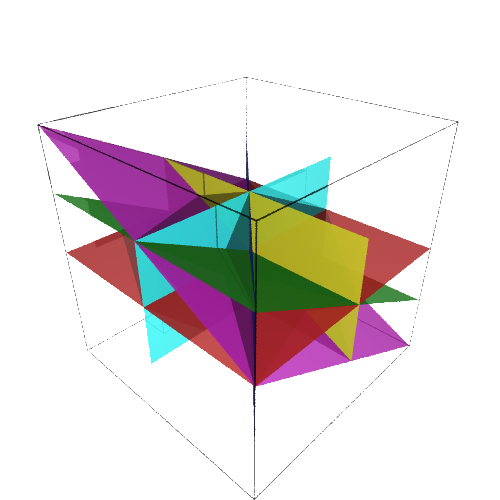
\includegraphics[width=0.4\textwidth]{graphics/Chap13SeparatingHyperplanes/Arrangement_hyperplans.png}
\caption[]{This awesome figure shows multiple (hyper)planes dividing $\real^3$ into disjoint regions, where each region could contain features describing a different object. In this book, we will content ourselves with a single hyperplane and do it in general for $\real^n$. Image courtesy of Kilom691 \url{ https://commons.wikimedia.org/w/index.php?curid=37508909}. } 
\label{fig:HyperplaneArrangment}
\end{figure}

We will develop the notion of a ``hyperplane'' as a linear object that is big enough to divide $\real^n$ into two halves, easy to manipulate, and can take on ``any orientation or position.'' In $\real^2$, any line can divide the space into two half spaces. In $\real^3$, a line is not ``big enough'' to divide the space into two parts, though the the classical notion of a plane does the job perfectly well. In $\real^n$, the appropriate generalization is called a \textbf{hyperplane}! \\

Before we dig into the details, we firm up concepts in $\real^2$. While we skip the case of the real line, $\real$, it does provide some insight because a single point $x_c \in \real$ can be used to divide the real line into two halves, $H^-:=\{x \in \real~| x < x_c\}$ and $H^+:=\{x \in \real~| x > x_c\}$. Moreover, the object being used to divide the vector space $\real$ into two halves has dimension zero, which is one less than the dimension of $\real$! Hold this thought.

\vspace*{0.2cm}


\begin{figure}[htb!]
    \centering
    \subfloat[]{%
	\centering
    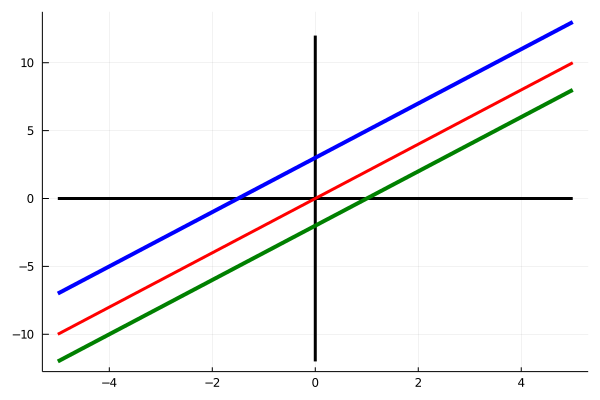
\includegraphics[width=0.48\columnwidth]{graphics/Chap13SeparatingHyperplanes/LinesTranslatedR2.png}
    }
      %\vspace{.2cm}
\subfloat[]{%
	\centering
  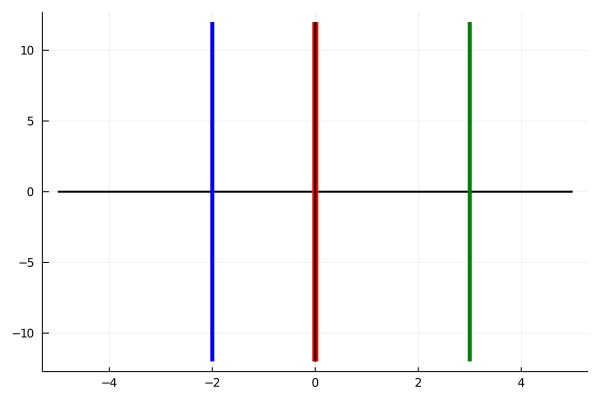
\includegraphics[width=0.48\columnwidth]{graphics/Chap13SeparatingHyperplanes/LinesTranslatedR2v02.png}
  }
    \caption[]{We know that subspaces must contain the origin. Lines in $\real^2$ can be viewed as translations of subspaces (loosely speaking, this means you slide them up, down, or sideways, without rotating them). In both figures, the lines corresponding to subspaces are in red while their translations are in green and blue. The blue and green lies are parallel to the red line, but are offset or translated. In (a),  the lines correspond to $0=a_0 + 1.0 x_1 -2.0 x_2$, where $a_0=0.0$ (red), $a_0=3.0$ (blue), and $a_0=-2.0$ (green) (b) The lines correspond to $0=a_0 + 1.0 x_1 + 0.0 x_2$, where $a_0=0.0$ (red), $a_0=2.0$ (blue) , and $a_0=-3.0$ (green)}
    \label{fig:MoreLinesR2}
    \end{figure}

\subsection{Lines in $\real^2$ as Separating Hyperplanes}
\label{sec:LineAsHyperplanes}

While we are very used to describing lines as things that satisfy formulas of the form $x_2 = mx_1+b$, let's note that this description leaves out the $x_2$-axis, which is a perfectly fine line in $\real^2$. It also leaves out all lines parallel to the $x_2$-axis. Why is the $x_2$-axis not covered by this description? Because it's slope would be infinity, which is not allowed! A better way to describe a line is actually as a special kind of subset of $\real^2$, such as 
$$ {\rm Line}:=\{ (x_1,x_2) \in \real^2~|~a_0 + a_1 x_1 + a_2 x_2  = 0 \}, $$
where at least one of $a_1$ and $a_2$ is non-zero. Indeed, with this formulation,
$$x_2\text{-axis} = \{ (x_1,x_2) \in \real^2~|~0 + x_1 + 0 x_2= 0 \}.  $$

% Said another way, it is the null space of 
% $$ C = \left[1~~0  \right]. $$

\textbf{Claim 1:} Every line in $\real^2$ can be written as the zero set of $y(x_1,x_2)=a_0 + a_1 x_1 + a_2 x_2$, where at least one of $a_1$ and $a_2$ is non-zero.\\

\textbf{Proof:} If the line is given by $x_2 = m x_1 + b$, then it is the zero set of $y(x_1,x_2)=b+m x_1 - x_2$, that is, $a_0=b$, $a_1=m$ and $a_2=-1.$ If the line is parallel to the $x_2$-axis, as in $ \{(x_1, x_2)~|~ x_1=a_0 = \text{a constant}, x_2 \in \real  \},$ 
then we can take  $y=a_0 - x_1 + 0 x_2$, that is,  $a_1=-1$ and $a_2=0.$
\Qed

\vspace*{0.2cm}

While it may not be apparent that writing a line as the zero set of a function has any value, we next note that the function  
$$y(x_1,x_2)=a_0 + a_1 x_1 + a_2 x_2$$
can also be used to divide $\real^2$ into two halves. Indeed, we define
\begin{align*}
H^+&:=\{(x_1, x_2) \in \real^2~|~ y(x_1,x_2) = a_0 + a_1 x_1 + a_2 x_2 >0\}\\
 H^-&:=\{(x_1, x_2) \in \real^2~|~ y(x_1,x_2) = a_0 + a_1 x_1 + a_2 x_2 <0\}.
\end{align*}
This is illustrated in Fig~\ref{fig:HalfSpacesR2}, where the line in red is the set where $y(x_1,x_2) = a_0 + a_1 x_1 + a_2 x_2 =0,$ showing the utility of thinking of a line as a zero set of a function.\\

\vspace*{.2cm}
\begin{tcolorbox}[sharp corners, colback=green!30, colframe=green!80!blue,title=\textbf{$H^+$ and $H^-$ are Called Half Spaces}]
$H^+$ and $H^-$ are called Half Spaces because they divide $\real^2$ into two halves. Is that really possible? In Fig~\ref{fig:HalfSpacesR2}, the red lines are the sets where $y(x_1,x_2) = a_0 + a_1 x_1 + a_2 x_2 =0$. We indicated $H^+$ and $H^-$ as being on opposite sides of the red lines. Does it have to be this way? Can these sets be mixed up, meaning parts of $H^+$ and $H^-$ can be on the same side of the red line? The answer is a \textbf{DEFINITIVE NO!} One side of the red line will be $H^+$ and the other will necessarily be $H^-$. To determine which is which, just sample one point on one of the sides and check if $y$ at that point is positive or negative. It's that simple. \\

Following this box, we give the optional proof. 
\end{tcolorbox}

\vspace*{.2cm}

\textbf{(Optional) Proof that Half Spaces Work as we Claim:} Here is why the line $y(x_1,x_2)=0$ separates $\real^2$ into \textbf{two half spaces, $H^+$ and $H^-$}.\\

Suppose that $(x^+_1,x^+_2) \in \real^2$ is such that $y^+:=y(x^+_1,x^+_2) >0$ and similarly, $(x^-_1,x^-_2) \in \real^2$ is such that $y^-:=y(x^-_1,x^-_2) < 0$. Let $\alpha \in \real$ and define a new point $(x_1(\alpha), x_2(\alpha) \in \real^2$ by
$$ \begin{bmatrix}x_1(\alpha)\\ x_2(\alpha)  \end{bmatrix}:= (1-\alpha) \begin{bmatrix}x^+_1 \\x^+_2  \end{bmatrix} +  \alpha \begin{bmatrix}x^-_1 \\ x^-_2 \end{bmatrix}. $$
We note that varying $\alpha \in \real$ traces out a line in $\real^2$ that passes through $(x^+_1,x^+_2)$ when $\alpha=0$ and through $(x^-_1,x^-_2)$ when $\alpha=1$.\\

We next note that we can write $y(x_1,x_2)$ as
$$y(x_1,x_2) = a_0 + a_1 x_1 + a_2 x_2 = a_0 +\left[ a_1~~~a_1  \right]  \begin{bmatrix}x_1\\ x_2 \end{bmatrix} $$
and therefore,
\begin{align*}
y(x_1(\alpha),x_2(\alpha)) &= a_0 +\left[ a_1~~~a_1  \right]  \begin{bmatrix}x_1(\alpha)\\ x_2(\alpha)  \end{bmatrix} \\
&= (1-\alpha) a_0 + (1-\alpha) \left[ a_1~~~a_1  \right] \begin{bmatrix}x^+_1 \\x^+_2  \end{bmatrix} +  \alpha a_0 + \alpha \left[ a_1~~~a_1  \right]  \begin{bmatrix}x^-_1 \\ x^-_2 \end{bmatrix}\\
&= (1-\alpha)y(x^+_1,x^+_2) + \alpha y(x^-_1,x^-_2) \\
&= (1-\alpha)y^+ + \alpha y^-. 
\end{align*}
Solving for $\alpha^*$ to set $y(x_1(\alpha^*),x_2(\alpha^*))=0$ yields
$$\alpha^* = \frac{y^+}{y^+ - y^-} =  \frac{y^+}{y^+ + |y^-|}, $$
where we have used the fact that $y^-<0 \implies -y^- = |y^-|.$ Because $|y^-|>0$ it follows that $0 < \alpha^* < 1$. Hence, there is a unique point $(x_1(\alpha),x_2(\alpha))$ \textbf{strictly between} $(x^+_1,x^+_2)$ and $(x^-_1,x^-_2)$ where $y(x_1(\alpha),x_2(\alpha))=0$. All points where $y(x_1,x_2)$ vanishes lie on a red line. Hence, the point $(x_1(\alpha^*),x_2(\alpha^*))$ lies on a red line. The only way this can happen is if $(x^+_1,x^+_2)$ and $(x^-_1,x^-_2)$ lie on opposite sides of a red line. \Qed

\vspace*{.2cm}

In the next subsection, we want to extend these ideas to $\real^n$ for $n >2$. While we could stick with formulas of the form 
\begin{equation}
\label{eq:SimpleFormulaPlane}
    y(x_1, \ldots, x_n) = a_0 + a_1 x_1 + \cdots + a_n x_n,
\end{equation} 
a more insightful analysis comes about from working directly with subspaces, which was hinted at in Fig.~\ref{fig:HyperplaneArrangment} and \ref{fig:MoreLinesR2}. 


\vspace*{.2cm}
\begin{figure}[bht!]
    \centering
    \subfloat[]{%
	\centering
    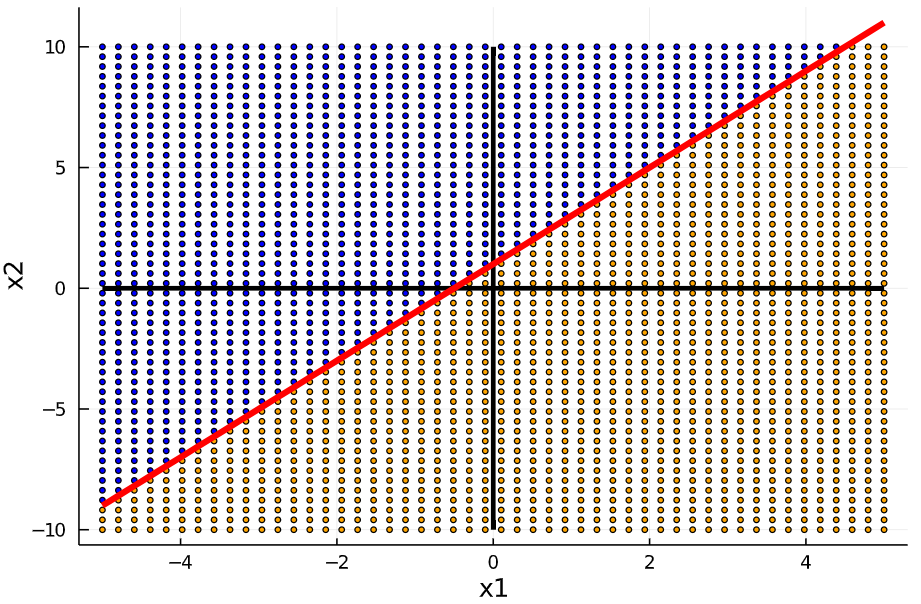
\includegraphics[width=0.48\columnwidth]{graphics/Chap13SeparatingHyperplanes/HalfPlanesR2_v01.png}
    }
      %\vspace{.2cm}
\subfloat[]{%
	\centering
  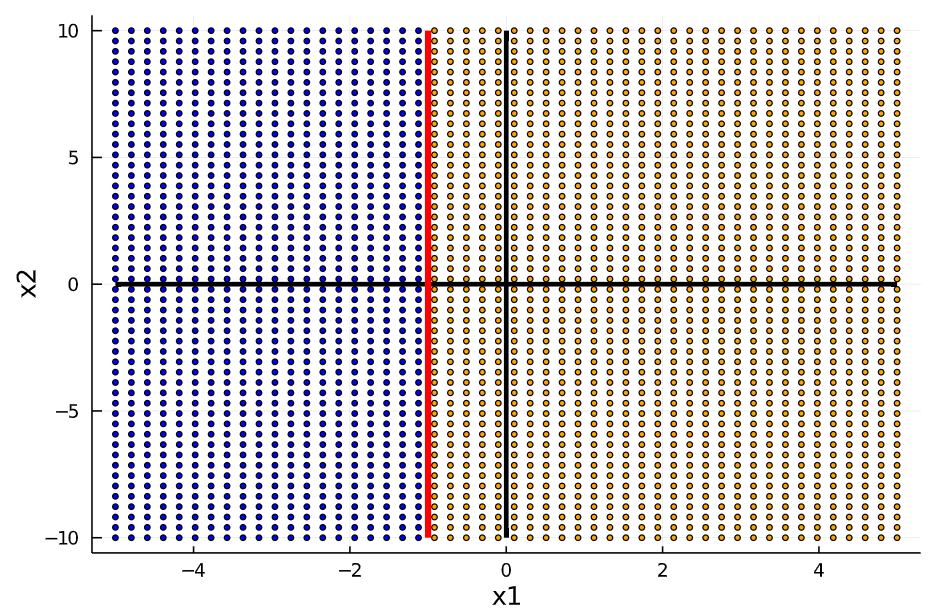
\includegraphics[width=0.48\columnwidth]{graphics/Chap13SeparatingHyperplanes/HalfPlanesR2_v02.png}
  }
    \caption[]{Two examples of half spaces corresponding to (a) $y=-1.0 -2.0 x_1 + x_2$ (b) $y=-1.0 -1.0 x_1 + 0.0 x_2$.  The line $y=a_0 + a_1 x_1 + a_2 x_2=0$ is shown in red, while in blue is plotted the set where $y > 0$ and in brown and the set where $y < 0$. The $x_1$-axis and $x_2$-axis are in black. 
    }
    \label{fig:HalfSpacesR2}
    \end{figure}


\subsection{Hyper Subspaces}

Consider the vector space $\real^n$ and let $A$ be a $1 \times n$ matrix (you can also call it a row vector). We assume that $A$ is non-zero, meaning that at least one of its components is non-zero. Viewing $A$ as a matrix, we know that its null space 
$$N:=\nullspace(A)=\{ x \in \real^n~|~Ax = 0 \} $$
is a subspace of $\real^n$. By the \textbf{Rank-Nullity Theorem}, the dimension of $N$ is equal to $n-1$, one less than the dimension of $\real^n$. Why, because $\rank(A)=1$ due to our assumption that at least one of its columns\footnote{For a $1 \times n$ matrix, elements and columns are the same thing!} is nonzero and
$$\dim(N) = \nullity(A) = \dim(\real^n) -\rank(A) = n -1. $$
A subspace with dimension one less than the ambient space in which it lives, which in our case is $\real^n$, is called a \textbf{co-dimension one} subspace. Though less common, you can also call it a \textbf{hyper-subspace}! \\

We've just seen that the null space of a rank one matrix gives rise to a co-dimension one subspace. Are all co-dimension one subspaces the null space of some matrix? The answer is yes and the easiest way to show it is by using the dot product and the Gram-Schmidt process! What? You did not see that coming? \\

We write $A=: a^\top$ where 
$$a:=\left[ \begin{array}{c} a_1 \\ a_2 \\ \vdots \\ a_n   \end{array} \right] \in \real^n .$$
We do this because 
$$ x \in \nullspace(A) \iff Ax=0 \iff  a^\top x =0 \iff  a \bullet x = 0 \iff  x \bullet a =0 \iff  x \perp a.  $$
Hence, our question of whether every co-dimension one subspace can be expressed as the null space of a rank one matrix can be rephrased as ``is every co-dimension one subspace equal to the set of all vectors that are orthogonal to a non-zero vector $a\in \real^n$?'' To answer this question, we can invoke Gram-Schmidt. \\

We let $N \subset \real^n$ be a co-dimension one subspace, meaning $\dim(N)=n-1$. We let $\{ u_1, \ldots, u_{n-1} \}$ be a basis for $N$. Because $N$ is not all of $\real^n$, there must exist a non-zero vector $u_n\in \real^n$ such hat $u_n \not \in N$. We skip the details, but you can then show that $$\{ u_1, \ldots, u_{n-1}, u_n \}$$
is a linearly independent set. We apply Gram-Schmidt to produce an orthogonal basis $\{ v_1, \ldots, v_{n-1} , v_n\}$. By \eqref{eq:SpanPreserving}, we have that
$$ N = \spanof{u_1, \ldots, u_{n-1}} = \spanof{v_1, \ldots, v_{n-1} }. $$
Moreover,
$$x \in N \iff x=\alpha_1 v_1 + \cdots \alpha_{n-1} v_{n-1} \iff x \perp v_n \iff v_n \bullet x = 0$$
\vspace*{.2cm}
\begin{tcolorbox}[title=\textbf{Hyper Subspaces and Dot Products}]
The following are equivalent for a subspace $N \subset \real^n$:
\begin{itemize}
    \item $\dim(N)=n-1$, that is, $N$ is a co-dimension one subspace;
    \item there exists $a\in \real^n$ not equal to zero such that $x\in N \iff x \perp a$; and
    \item there exists a $1 \times n$ matrix $A$ such that $A \neq 0_{1 \times n}$ and $N=\nullspace(A)$.
 \end{itemize}
   
\end{tcolorbox}
\vspace*{.2cm}

We note that the matrix $A$ and the vector $a$ are related by $A=a^\top$.

\vspace*{.2cm}

\begin{example}
\label{ex:CoDimensionOneSubspace}
Consider a matrix $B=\left[ \begin{array}{rr} 1 & -1 \\ -1 & 2 \\ 0 & 1\end{array} \right] $ and let $N:=\colspanof{B}$. It is clear that $N \subset \real^3$ and $\dim(N)=2$. Find a vector $a\in \real^3$ such that 
$$N=\{ x\in \real^3~|~ a\bullet x = 0 \}. $$
\end{example}

\textbf{Solution:} We define $u_1=\left[ \begin{array}{r} 1 \\ -1 \\ 0 \end{array} \right] $, $u_2=\left[ \begin{array}{r} -1 \\ -2 \\ 1 \end{array} \right] $, and note that $u_3=\left[ \begin{array}{r} 1 \\ 1 \\ 0 \end{array} \right] $ is linearly independent of $\{ u_1, u_2\}$. Applying Gram Schmidt with normalization to $\{ u_1, u_2, u_3  \}$ yields
$$\left[ \begin{array}{ccc} v_1 & v_2 & v_3 \end{array} \right] = \left[ \begin{array}{rrr}  0.707107 & 0.408248  & 0.57735 \\
 -0.707107 & 0.408248 &  0.57735 \\
  0.000000 &0.816497  & -0.57735 \end{array} \right]. $$
  Hence, we can take $a=\left[ \begin{array}{r} 1 \\ 1 \\ -1\end{array} \right]$. It is easily checked that $a \bullet u_1= 0$ and $a \bullet u_2 = 0$, and thus $N=\{ x\in \real^3~|~ a\bullet x = 0 \}$. 
 \Qed


\begin{figure}[htb!]
    \centering
    \subfloat[]{%
	\centering
    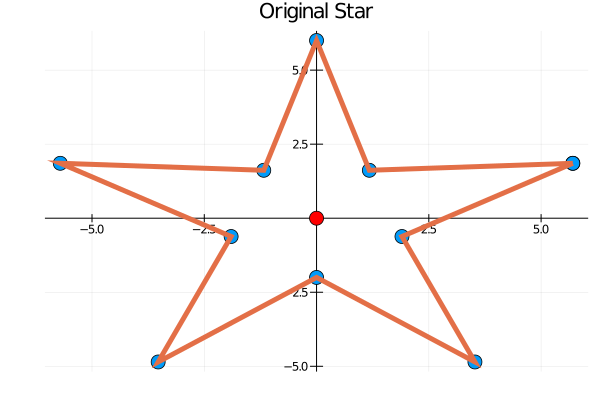
\includegraphics[width=0.48\columnwidth]{graphics/Chap13SeparatingHyperplanes/StarOriginal.png}
    }
      %\vspace{.2cm}
\subfloat[]{%
	\centering
  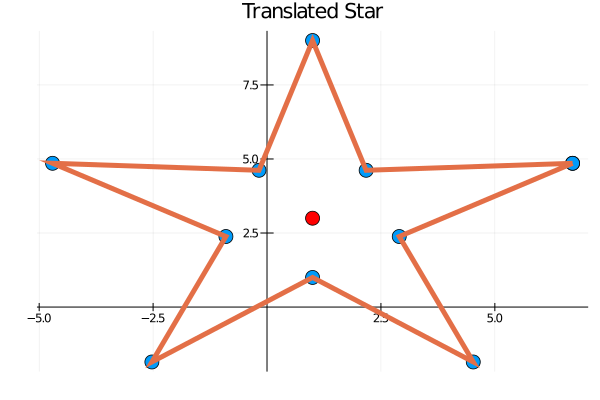
\includegraphics[width=0.48\columnwidth]{graphics/Chap13SeparatingHyperplanes/StarTranslated.png}
  }
    \caption[]{Let $S\subset \real^2$ be the star-shaped object in (a) and let $x_c$ be the vector $[2; 3]$. Then $x_c + S$ is the star-shaped object in (b), where each and every point of the object has been shifted by $x_c$. If you can handle this, then you should have no trouble handling the translation of a line or a plane! Image courtesy of Tribhi Kathuria.}
    \label{fig:TranslationStar}
    \end{figure}

\subsection{Translations of Sets, Hyper Subspaces, and Hyperplanes}

\textbf{Definition} Let $S\subset \real^n$ be a subset and and let $x_c\in \real^n$ be a vector. We define the translation of $S$ by $x_c$ as
$$ x_c + S:= \{x_c + x~|~ x\in S \}.$$
Note that, because $S$ consists of vectors in $\real^n$, the addition in the above formula makes sense. Figure~\ref{fig:TranslationStar} provides an illustration. 


\vspace*{0.2cm}
    
\textbf{Claim:} Let $N = \{ x\in \real^n~|~ a \bullet x = 0\} \subset \real^n$ be a hyper subspace (means that $a \neq 0_{n \times 1}$) and let $x_c\in \real^n$ be a vector. Then their sum has a simple description as
\begin{equation}
    \label{eq:DefHyperPlaneEq}
   x_c + N =\{ x\in \real^n~|~ a \bullet(x-x_c)=0\} = \{ x\in \real^n~|~ a \perp (x-x_c)\}.
\end{equation}

The proof is not important, but we give it for those who are interested. $N$ consists of everything in $\real^n$ that is orthogonal to $a$. Hence, if $(x-x_c) \perp a$, then $(x-x_c) \in N$. Adding $x_c$ to both sides, we have that $x \in x_c + N$. The other direction is similar. \Qed

    \vspace*{0.2cm}

\begin{tcolorbox}[title=\textbf{Hyperplanes are Translations of Hyper Subspaces}]
Let $N = \{ x\in \real^n~|~ a \bullet x = 0\} \subset \real^n$ be a hyper subspace (means that $a \neq 0_{n \times 1}$) and let $x_c\in \real^n$ be a vector. Then 
\begin{equation}
    \label{eq:DefHyperPlane}
    H:=x_c + N 
\end{equation}
is called a \textbf{hyperplane}. Moreover, by \eqref{eq:DefHyperPlaneEq}, the real-valued function $y:\real^n \to \real$ defined by
\begin{equation}
    \label{eq:DefHyperPlaneFunction}
    y(x):=a \bullet(x-x_c)
\end{equation}
vanishes on $H=x_c + N$ (because $ H =\{x\in \real^n~|~y(x)= a\bullet(x-x_c) =0\})$. It follows that $y(x)$ can be used to divide $\real^n$ into two halves
\begin{equation}
    \label{eq:halfSpaces}
    \begin{aligned}
        H^+&:= \{ x\in \real^n~|~ y(x) > 0\} \\
        H^-&:= \{ x\in \real^n~|~ y(x) < 0\}.
    \end{aligned}
\end{equation}
A fanciful illustration is given in Fig.~\ref{fig:SeparatingHyperplane}.\\

We note that $H^+$ is the set of all vectors $x\in \real^n$ such that the dot product $ <a,  x-x_c > = a \bullet (x-x_c) >0$, while $H^-$ is the set of all vectors $x\in \real^n$ such that $<a,  x-x_c > = a \bullet (x-x_c) <0$. 
\end{tcolorbox}
 
  \vspace*{0.2cm}
  
\textbf{Remarks:} 
\begin{itemize}
\item Without loss of generality, it is always possible to take $x_c = \alpha a$, for $\alpha \in \real.$ Indeed, one can go back and forth between \eqref{eq:DefHyperPlaneFunction} and \eqref{eq:SimpleFormulaPlane} by
  \begin{equation}
      \label{eq:HyperplaneEquivalentFormulas}
      a_0 = - a \bullet x_c~~\text{and}~~x_c = - a_0 \frac{a}{||a||^2}
  \end{equation}
  \item Vectors such that $<a,  x-x_c > = a \bullet (x-x_c) > 0$ form an \textbf{acute angle (less than $90^o$)} with respect to the vector $a$, while vectors such that $<a,  x-x_c > = a \bullet (x-x_c) < 0$ form an \textbf{oblique angle (greater than $90^o$)} with respect to the vector $a$. Vectors such that $<a,  x-x_c > = a \bullet (x-x_c) = 0$ form a \textbf{right angle (exactly $\pm 90^o$)} with respect to the vector $a$, and hence are on the hyperplane itself.
\end{itemize}

 \vspace*{0.2cm}
\begin{figure}[hbt!]
\centering
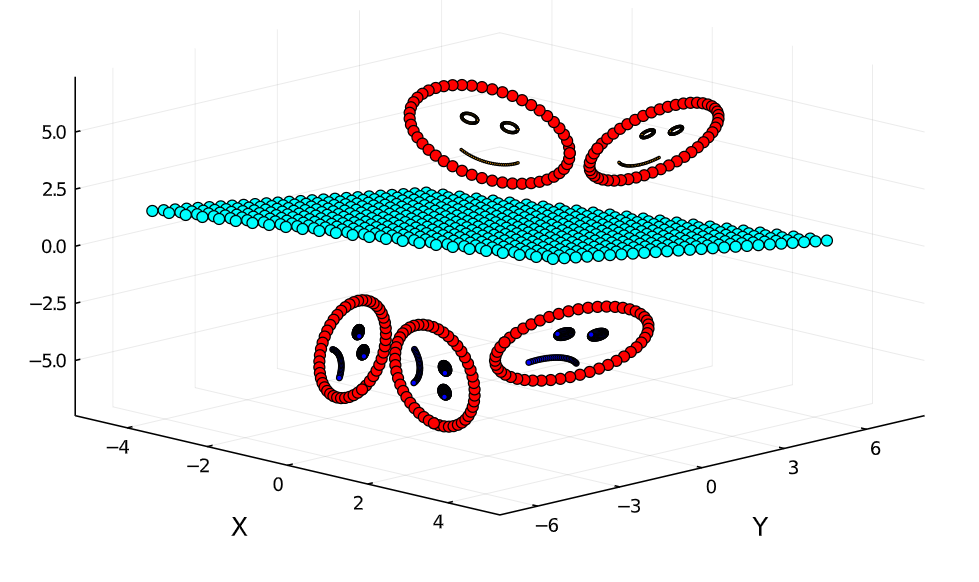
\includegraphics[width=0.6\textwidth]{graphics/Chap13SeparatingHyperplanes/SeparatingHyperPlaneSmileFrown.png}
\caption[]{A separating hyperplane where the features are smiles versus frowns. In Example~\ref{ex:MaxMarginClassifier}, we show how to design the parameters of the hyperplane, that is,  $a\in \real^n$ and $x_c \in \real^n$, so as to achieve separation for given data on the features.} 
\label{fig:SeparatingHyperplane}
\end{figure}

\section{Signed Distance to a Hyperplane}
\label{sec:SignedDistance}

% This section seeks to tie together Chapters~\ref{sec:SeparatingHyperplanes} and \ref{sec:OrthogonalProjection}. The material is used in Machine Learning EECS 445. While we doubt it is taught in Math 214, we'll cover it here because we know from Prof. Sindhu that it will help you.

% \subsection{Signed Distance to a Hyperplane}

The function $y(x)= a\bullet (x-x_0)$ has another amazing feature: its absolute value is proportional to the distance of a point $x$ from the hyperplane $H^0$ defined by $H^0:=\{ x \in \real^n~|~y(x)=0 \}$. Moreover, $y(x)$ gives rise to the notion of the signed distance of $x$ to $H^0$ because, depending on which of the half-planes $x$ lies, the sign of $y(x)$ will be either $+1$ or $-1$. To make sense of this, we must first define the distance of a point to a subspace, and then we will specialize to the case that the subspace is a hyper-subspace.\\

\begin{tcolorbox}[title=\textbf{From Norms to Distances}]
Let $V\subset \real^n$ be a subspace and let $x_0\in \real^n$, $y_0\in \real^n$, $v_c\in \real^n$ be points. Then 
\begin{itemize}
    \item \textbf{Definition} $d(x_0, y_0):=||x_0 - y_0 ||$ is called the \textbf{distance} from $x_0$ to $y_0$.
    \item  \textbf{Definition} $d(x_0,V):=\min\limits_{v \in V} ||x_0 - v ||$ is called the \textbf{distance} from $x_0$ to $V$.
\end{itemize}
The translation of a subspace by vector is called a \textbf{linear variety}. Let $W:=v_c + V$. Then one can also define
\begin{itemize}
    \item \textbf{Definition} $d(x_0,W):=\min\limits_{w \in W} ||x_0 - w ||$ is called the \textbf{distance} from $x_0$ to $W$.
    \end{itemize}
\end{tcolorbox}

\textbf{Fact:} If $W=v_c+V$, then $d(x_0, W)=d(x_0-v_c,V)$.
\vspace*{0.2cm}

The somewhat amazing fact is that when $V$ is a hyperplane, the minimization problem defining the distance of a point to the hyperplane has a very simple solution! \textcolor{red}{This only works for hyperplanes, that is, linear varieties that are translates of hyper subspaces.}

\vspace*{0.2cm}

\begin{tcolorbox}[sharp corners, colback=green!30, colframe=green!80!blue, title=\textbf{\large Signed Distance to a Hyperplane}]
Suppose that $y:\real^n \to \real$ is given by \eqref{eq:SimpleFormulaPlane} or \eqref{eq:DefHyperPlaneFunction} and that $a \neq 0_{n \times 1}$ (recall that one can go back and forth between the two representations by \eqref{eq:HyperplaneEquivalentFormulas}). Let
$H^0:=\{x \in \real^n~|~ y(x) = 0 \}$ be the hyperplane defined by $y$. Then, for all $x_0 \in \real^n$,
$$ |y(x_0)|= ||a||~d(x_0, H^0), $$
that is, 
$$d(x_0, H^0) = \frac{|y(x_0)|}{||a||} $$
For this reason, 
\begin{equation}
\label{eq:SignedDistance}
\frac{y(x)}{||a||}
\end{equation}
is called the \textbf{signed distance} from $x$ to $H^0$. 

\end{tcolorbox}

\vspace*{0.2cm}

\begin{example}
\label{ex:SignedDistance01} Compute the signed distance for a hyperplane defined by
$$P:=\{(x_1, x_2) \in \real^2~|~ 1.5 x_1 - 2.0 x_2 = -4.0\}. $$
\end{example}

\textbf{Solution} We have the hyperplane is defined by $y:\real^2 \to \real$, where 
$$y(x_1,x_2)= 1.5 x_1 - 2.0 x_2 + 4.0 .$$
Hence, $a=[1.5; -2.0]$ and 
 $$\frac{1}{||a||}y(x_1,x_2)=\frac{1.5 x_1 - 2.0 x_2 + 4.0}{\sqrt{6.25}}$$ is the signed distance from $x=\begin{bmatrix}
x_1\\x_2
\end{bmatrix}$ to the hyperplane $P$.

\Qed

\vspace*{0.2cm}

\begin{example}
\label{ex:SignedDistance02} Compute the signed distance for a hyperplane defined by
$$P:=x_c + \{ x \in \real^n~|~ x \perp a\}. $$
\end{example}

\textbf{Solution} We know that the hyperplane is defined by $y:\real^n \to \real$, where 
$$y(x)=a\bullet(x-x_c).$$
Hence, $y(x)=\frac{a}{||a||}\bullet(x-x_c)$ gives the signed distance. 
\Qed

\vspace*{0.2cm}

\begin{example}
\label{ex:SignedDistance03} For a $d$-dimensional hyperplane that passes through the origin and is defined by the normal vector $[a_1;a_2; \ldots, a_d]$, compute the signed distance function.
\end{example}

\textbf{Solution} We know that the hyperplane is defined by $y:\real^d \to \real$, where 
$$y(x)=a\bullet x$$
Hence, $y(x)=\frac{a\bullet x}{||a||}$ is the signed distance function.
\Qed


\begin{example}
\label{ex:exampleSignedDistanceProof} Prove the signed distance formula, namely, 
\begin{equation}
\label{eq:SignedDistanceFormula}
    |y(x_0)| = ||a|| ~d(x_0, H^0)  
\end{equation}

\end{example}

\textbf{Solution} The proof uses a few ideas we have not covered in ROB 101, so will only sketch it. So that the hyperplane is well defined, we assume that $a \in \real^n$ is not the zero vector and that 
\begin{equation}
\label{eq:TranslateOfHypersubspace}
    H^0:=\{x\in \real^n~|~a\bullet(x - x_c)=0 \} = x_c + N, \text{ where } N:=\{x\in \real^n~|~a \bullet x=0 \}.
\end{equation}

Because $a \neq 0_{n \times 1}$ and $N$ is the set of all vectors (points) orthogonal to $a$, it follows that every vector in $\real^n$ can be written as a multiple of $a$ and a vector in $N$. In particular, we have that 
\begin{align*}
    x_c = & \alpha a + \overline{x} \text{ for some } \alpha \in \real \text{ and } \overline{x} \in N\\
    & \text{ and for all } x\in \real^n \\
    x  = &\beta a  + \doverline{x} \text{ for some } \beta \in \real \text{ and } \doverline{x} \in N. 
\end{align*}

Using the above relations, we first evaluate 
\begin{align*}
    |y(x)| & = | a \bullet (x - x_c) | \\
    & =  | a \bullet (\alpha a + \overline{x} - \beta a  - \doverline{x}) | \\
    & = |\alpha -\beta|~ ||a||^2
\end{align*}
where we used two facts: (i) $a \bullet \overline{x} = 0$ and  $a \bullet \doverline{x} = 0$ because $\overline{x}, \doverline{x} \in N$ and (ii) $a \bullet a = ||a||^2$ for the Euclidean norm.\\

Next, we observe that 
\begin{align*} 
    d^2(x, H^0) & = \min_{\widetilde{x} \in H^0} || x - \widetilde{x}||^2 \\
    & =  \min_{\widetilde{x} \in N} || x - (\widetilde{x} + x_c)||^2 \\
    & =  \min_{\widetilde{x} \in N} || (\beta a  + \doverline{x} ) - (\widetilde{x} + \alpha a + \overline{x})||^2 \\
    & =  \min_{\widetilde{x} \in N} || (\beta   - \alpha )a + (\doverline{x} - \widetilde{x} - \overline{x})||^2 \\
    & =  \min_{\widetilde{x} \in N} \left[ ||  (\beta  - \alpha)a||^2  + || \doverline{x} - \widetilde{x} - \overline{x}||^2 \right] \\
    & = |\beta  - \alpha|^2 | ~||a||^2 +  \min_{\widetilde{x} \in N} || \doverline{x} - \widetilde{x} - \overline{x}||^2 \\
    & = |\beta  - \alpha|^2 | ~||a||^2,
\end{align*}
where we used the Pythagorean Theorem to arrive at 
$$|| (\beta   - \alpha )a + (\doverline{x} - \widetilde{x} - \overline{x})||^2  =  ||  (\beta  - \alpha)a||^2  + || \doverline{x} - \widetilde{x} - \overline{x}||^2  = $$
and we noted that
$$  \min_{\widetilde{x} \in N} || \doverline{x} - \widetilde{x} - \overline{x}||^2 = 0,$$
because $\doverline{x} - \overline{x} \in N$. Hence, taking square roots, 
$$ d(x, H^0) = |\beta  - \alpha|~  ~||a||. $$
Comparing the formulas for $d(x, H^0)$ and $|y(x)|$ we arrive at 
$$ |y(x)| = ||a||~d(x, H^0).$$
\Qed

\begin{figure}[hb!]%
\centering
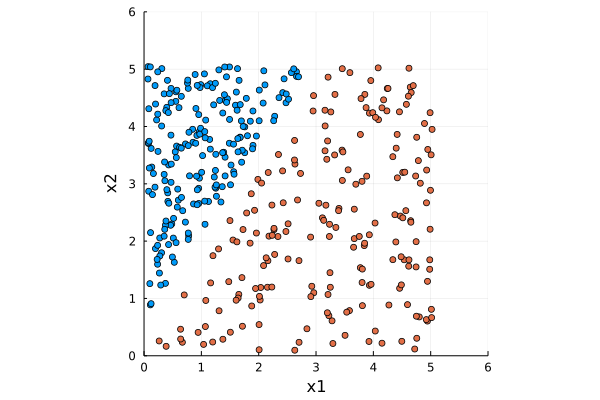
\includegraphics[width=0.95\columnwidth]{graphics/Chap13SeparatingHyperplanes/MaxMarginClassifierRawData.png}%
\caption[]{Raw data for a maximum margin classifier The blue data will be Class 1, labeled with a $+1$, and the red data will be Class 2, labeled with a $-1$. 
}    
\label{fig:max_margin_gt}
\end{figure}

%\vspace*{0.2cm}

\section{Max-margin Classifier}
\label{sec:MaxMarginClassifier}

\textcolor{blue}{\bf This material is from lectures in ROB 101 given by Prof. Maani Ghaffari.}\\

In the next example, we will formulate a (linear) classifier to separate points that belong to two different categories called \textbf{class labels}. For example, you can think of this as a model that predicts whether an email is spam or not.  Our model is linear and separates the space into two half-spaces, as described in Chap.~\ref{sec:SeparatingHyperplanes}. As shown in Chap.~\ref{sec:LineAsHyperplanes}, in the 2D plane, a line divides the space into two half-spaces. In general, we will be designing a \textbf{separating hyperplane}, that is, a translation of a co-dimension one subspace.\\

\textbf{Definition:} Consider a labeled data set $\mathcal{D} = \{(x_i,\ell_i)\}_{i=1}^n$, where $x_i \in \real^m$ and $\ell_i = \pm 1$, and suppose that $H :=\{x \in \real^m~|~ y(x) = 0 \}\subset \real^m$ is a hyperplane. Then $H$ \textbf{separates the data}, if for each $1 \le i \le n$, (i) $y(x_i) \neq 0$ (no data points lie on the hyperplane) and (ii) ${\rm sign}~~y(x_i) = \ell_i$ (the sign of the label $\ell_i$ determines on which side of the hyperplane the data point $x_i$ lies). Then the \textbf{margin} is defined to be
\begin{equation}
\label{eq:marginDef}
{\rm margin}:= \underset{x_i, \ell_i = +1}{\min} d(x_i, H) + \underset{x_j, \ell_j = -1}{\min} d(x_j, H)
\end{equation}
   
\Qed

\begin{remark}  \textcolor{red}{\bf Intuitively, the larger the margin, the more robust the separation (aka classification) of the data. } We can evaluate the distances used to define the margin by $|y(x_i)|/||a||$. Hence, 
\begin{equation}
\label{eq:marginDef02}
{\rm margin}:= \underset{x_i, \ell_i = +1}{\min} \frac{|y(x_i)|}{||a||} + \underset{x_j, \ell_j = -1}{\min} \frac{|y(x_j)|}{||a||} = \frac{1}{||a||} \left(\underset{x_i, \ell_i = +1}{\min} |y(x_i)| + \underset{x_j, \ell_j = -1}{\min} |y(x_j)|\right).
\end{equation}
We note that if $|y(x_i)|\ge 1$ for all $1\le i \le n$, then 
$$ {\rm margin} \ge \frac{2}{||a||}.$$ And if there is at least one point in each class such that $|y(x_i)|=1$, then the margin is exactly equal to $ \frac{2}{||a||}$. In that case, maximizing the margin is the same as minimizing $||a||$. Vectors such that $|y(x_i)|=||a|| ~ d(x_i, H)$ are called \textbf{support vectors}. 
\end{remark}


\begin{example}[Maximum Margin Classifier]
\label{ex:MaxMarginClassifier}
Given a labeled data set $\mathcal{D} = \{(x_i,\ell_i)\}_{i=1}^n$, find, if possible, a separating hyperplane that maximizes the margin. This problem appears in machine learning and is called the max-margin classifier. The goal is to build a linear model $y(x) = a \bullet x + a_0$ that can separate the two classes of data with the maximum margin possible. 

\end{example}

\textbf{Solution:}

Figure~\ref{fig:max_margin_gt} shows a synthetic data set (means we generated it in a computer) with red circles and blue crosses. To generate the data, we defined the line $\bf x_2 = 1.5 x_1 + 0.4$ as our \textbf{ground truth} and randomly generated vectors in $\real^2$: if they landed above the line, we labeled them with red circles; and if they fell below the line, we labeled them with blue circles. Synthetic data generated in this manner is how one tests a problem formulation and solution in practice!\\

Problems such as this one are called toy examples. They are simple enough that we can visualize and track the solution to ensure our software works as expected. The green line in Fig.~\ref{fig:max_margin_dataPresentation} is the hyperline $\bf x_2 = 1.493 x_1 + 0.398$ we computed to separate the two classes of data. We let you know this ahead of time so that you will read on and see how we did it!\\


Our dataset consists of 2D vectors (called inputs), $x_i \in \mathbb{R}^2$, and class labels (called target or output), $\ell_i \in \{-1,+1\}$. If we have $n$ data points, we write the dataset as
$$\mathcal{D} = \{(x_i,\ell_i)\}_{i=1}^n.$$
From Chap.~\ref{sec:SeparatingHyperplanes}, the line (hyperplane) that separates the data can be written as 
$$y(x)= a^\top x + a_0 = 0,$$ for $a_0\in \real$ and $a \in \real^2$. We can also combine the normal vector, $a$, and the bias, $a_0$, into 
$$w := \begin{bmatrix} a \\ a_0 \end{bmatrix}^\top \in \mathbb{R}^3,$$ and append a one to the inputs as $\bar{x}_i:=\begin{bmatrix} x_i; 1 \end{bmatrix}$.
Then the side of the line (hyperplane in general) on which each data point lies can be written as
\begin{equation}
\label{eq:InequalityConstraintsMaxMargin}
\begin{aligned}
     w^\top \bar{x}_i &\geq ~~~1 \quad \text{if} \quad \ell_i = ~~~1,\\
     w^\top \bar{x}_i &\leq -1 \quad \text{if} \quad \ell_i = -1;
\end{aligned}    
\end{equation}
moreover, with this assignment, $|y(x_i)|\ge 1$ for all $1 \le i \le n$, and therefore,
$${\rm d}(H, x_i) \ge \frac{1}{||a||}$$
by \eqref{eq:SignedDistance}.  Hence, the margin is maximimized by minimizing $||a||$, or equivalently, minimizing $||a||^2 = a^\top a$.\\


\begin{figure}[t]%
\centering
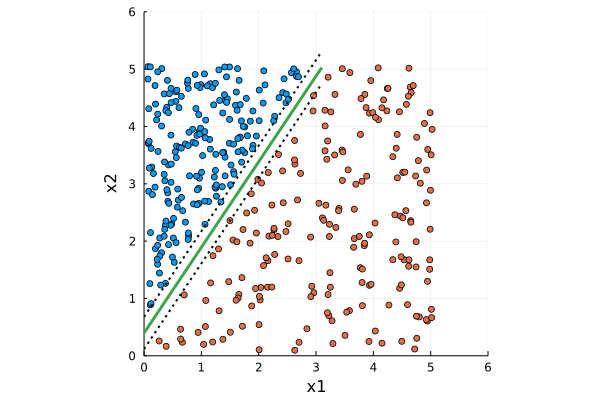
\includegraphics[width=0.95\columnwidth]{graphics/Chap13SeparatingHyperplanes/MaxMarginClassifierDataProcessed.png}%
\caption[]{The two classes are now separated by a hyperplane that provides the maximum margin, that is, the gap between the data points and the hyperplane. The code given below provides the optimal parameters $w^\ast = [-12.88, 8.42, -2.76]$, and thus $a^\ast = [-12.88, 8.42] $, $a_0^\ast = -2.76$, and the margin is $ 2 /||a^\ast = 0.31$. Moreover, any vectors that lie on either of the two dotted lines are the support vectors. There must be at least one vector in each class that lies on the lines, for if not, the line can be moved to increase the margin.
}    
\label{fig:max_margin_dataPresentation}
\end{figure}

The inequality constraints \eqref{eq:InequalityConstraintsMaxMargin} state that the data points for each class must lie on the correct side of the hyperplane for it to be a separating hyperplane! We can combine the two constraints into
\begin{equation}
\label{eq:MaxMarginCommonConstraint}
       \ell_i(w^\top \bar{x}_i) \geq 1, ~~1 \le i \le n.
\end{equation}
 

Finally, the problem can be formulated as the following QP:
   $$ \underset{ \begin{array}{c} \\  w = \left[\begin{array}{c} a \\ a_0 \end{array} \right] \in \real^3  \\
   \\
        \text{subject to  }   \ell_i(w^\top \bar{x}_i) \geq 1, \quad i = 1,\dots, n \end{array}  } { \min \frac{1}{2} \lVert a \rVert^2 } 
        $$         
After solving the problem, suppose ${w}^\ast = [a^\ast; a_0^\ast]$ is the optimal solution. We can predict the class label of a new input (called a query point), $x_{\rm data}$, by simply checking which side of the hyperplane it lies on
$$\text{class label is} \begin{cases} \text{(+1) blue circles} & a^\ast \bullet x_{\rm data} + a_0^\ast > 0 \\ \text{(-1) red circles} & a^\ast \bullet x_{\rm data} + a_0^\ast < 0 \end{cases}. $$
The results are shown in Fig.~\ref{fig:max_margin_dataPresentation}. \\

\Qed

\vspace*{.2cm}

\begin{tcolorbox}[sharp corners, colback=green!30, colframe=green!80!blue, title=\textbf{\large Highlights of the Max Margin Classifier for Two Classes}]

\begin{itemize}
    \item The process starts with a labeled data set $\mathcal{D} = \{(x_i,\ell_i)\}_{i=1}^n.$ Here we assume that $\ell_i \in \{-1, +1\} $ and $x_i \in \real^m$.
    \item The separating hyperplane is parameterized by $y(x)= a^\top x + a_0 = 0$, for $a_0\in \real$ and $a \in \real^m$. The hyperplane is $H:=\{x\in \real^m~|~ y(x) = 0\}$

    \item We write the constraints representing a point $x_i$ belonging to one of the two classes $\{-1, +1\}$ by $$\begin{aligned}
     w^\top \bar{x}_i &\geq ~~~1 \quad \text{if} \quad \ell_i = ~~~1,\\
     w^\top \bar{x}_i &\leq -1 \quad \text{if} \quad \ell_i = -1,
\end{aligned}  \iff \ell_i w^\top \bar{x}_i \ge 1, ~1 \le i \le n,$$ 
where $$ w = \left[ \begin{array}{c}a \\ a_0 \end{array} \right].$$

\item With the constraints written as above, the margin is greater than or equal to $\frac{2}{||a||}$, where $a\in \real^m$ is the normal vector defining the hyperplane. If there is a point in the data set such that $|y(x_i)|=1$, then $d(H,x_i) = 1/||a||$, and thus our estimate for the margin is tight. The bias term $a_0 \in \real$ provides the offset of the hyperplane so that it does not have to pass through the origin. Hence, to maximize the margin, we minimize $||a||$, subject to the classification constraints.

\item Putting all of this together leads to a Quadratic Program or QP as presented in Chapter~\ref{sec:QPs}:
   $$ \underset{\left[\begin{array}{c}  \ell_1 ~\bar{x}_1^\top \\ \vdots \\  \ell_n ~\bar{x}_n^\top \end{array} \right] \left[\begin{array}{c} a \\ a_0 \end{array} \right]  \geq {\bf \large 1}_{n \times 1}} { \min \frac{1}{2} a^\top a } 
        $$   

 \item Given a new data point $x_{\rm new} \in \real^m$, how do we determine its class? We evaluate $y(x_{\rm new} ) = a^\ast \bullet x + a_0$ and check its sign! If $y(x_{\rm new} )>0$, it is in Class 1 and if $y(x_{\rm new} )<0$, it is in Class 2.        
\end{itemize}

    
\end{tcolorbox}


\begin{lstlisting}[language=Julia,style=mystyle]
# # New Packages for solving QPs
# using Pkg
# Pkg.add("OSQP")
# Pkg.add("Compat")
using OSQP
using SparseArrays

# Standard Packages for ROB 101
using LinearAlgebra 
using Random
Random.seed!(123456);

# generate a dataset
N = 200
k1 = 0; # number of 1
k2 = 0; # number of -1
X = zeros(2*N,2) # input matrix
ell = zeros(2*N,1) # target values
i = 1;
marginDes = .3
while minimum([k1 k2]) < N
    x = rand(1,2) * 5. .+ .05;
    # separating line is x2 = 1.5 x1 + 0.4
    y = (x[2] - 1.5 * x[1] - 0.4)/norm([-1.5 1]); # norm of a = 1
    # generate target values
    if (y > marginDes/2.) && k1 < N
        ell[i] = 1;
        X[i,:] = x;
        k1 += 1;
        i += 1;
    elseif (y < -marginDes/2.) && k2 < N
        ell[i] = -1;
        X[i,:] = x;
        k2 += 1;
        i += 1;
    end
end

# Class +1 IDs
class1_id = ell.== 1;

using Plots
gr() # Set the backend to GR

plot(X[class1_id[:],1], X[class1_id[:],2], seriestype = :scatter, 
    aspectratio=:equal, legend=false)
plot!(X[.!class1_id[:],1], X[.!class1_id[:],2], seriestype = :scatter, xlims = (0,6), ylims = (0,6))
xlabel!("x1")
ylabel!("x2")
plot!(fmt = :png)

\end{lstlisting}
\textbf{Output} 
See Fig.~\ref{fig:max_margin_gt}.

\begin{lstlisting}[language=Julia,style=mystyle]
# Data for Max Margin in R^2

# Define problem data
Q = (zeros(3,3) + I); Q[3,3]=0
q = zeros(3,1);
Ain = -([ell ell ell] .* [X ones(size(X,1),1)]);
bin = -ones(size(X,1),1);
dimX=length(q)
Aeq = Array{SparseMatrixCSC,2}(undef,0,dimX) # Empty Matrix
beq = Vector{Float64}(undef,0)               # Empty Matrix
lb = Vector{Float64}(undef,dimX).-Inf        # - infinity means no hard lower bound
ub = Vector{Float64}(undef,dimX).+Inf        # + infinity means no hard upper bound

wStar = quadProg(Q,q,Ain,bin,Aeq,beq,lb,ub)
@show wStar
@show margin = 2.0/norm(wStar[1:2])
aStar = wStar/norm(wStar[1:2])

\end{lstlisting}
\textbf{Output} 
\begin{verbatim}
wStar = [-5.3085002098319585, 3.5545545440849087, -1.4143558513794734]
margin = 2.0 / norm(wStar[1:2]) = 0.31305447944860626
\end{verbatim}

\begin{lstlisting}[language=Julia,style=mystyle]
# Our lines have to be plotted as y = mx + b and not 
# as a[1]*x + a[2] * y + a[3]; 
# Hence, we must solve for x2

x_line = collect(0:0.1:3.1)
y_line = -(aStar[1] * x_line .+ aStar[3])/aStar[2]


pMMC = plot!(x_line, y_line, lw = 3)


y_marginPlus = -(aStar[1] * x_line .+ aStar[3] .+ margin/2)/aStar[2]
y_marginMinus = -(aStar[1] * x_line .+ aStar[3] .- margin/2)/aStar[2]
plot!(x_line, y_marginPlus, lw=2, ls=:dot, color=:black)
plot!(x_line, y_marginMinus, lw=2, ls=:dot, color=:black)
plot!(fmt = :png)

display(pMMC)
\end{lstlisting}
\textbf{Output} 
See Fig.~\ref{fig:max_margin_dataPresentation}.

\begin{tcolorbox}[title={\bf Now that you are warmed up ...}]
There are excellent tutorial videos available for many aspects of Machine Learning (ML). Here are a few related to SVMs:

\begin{itemize}
    \item \url{https://youtu.be/-Z4aojJ-pdg} (Under the hood of SVM)

    \item \url{https://youtu.be/vMmG_7JcfIc} (Intro to the Kernel Trick)

    \item \url{https://youtu.be/OKFMZQyDROI} (More advanced view of the Kernel Trick)

    \item \url{https://youtu.be/bM4_AstaBZo} (Math behind SVM)

    \item \url{https://youtu.be/kb4apnc2imA} (Multi-class SVM)
\end{itemize}
    
\end{tcolorbox}


\section{Remarks on Soft Margin Classifiers} 

\textcolor{blue}{\bf This material is from lectures in ROB 101 given by Prof. Maani Ghaffari.}\\

In real life, the data are rarely so nicely separated. There is almost always some overlaps, perhaps due to random errors and outliers, or perhaps because some valid emails look a lot like spam! 


\begin{figure}[hb!]%
\centering
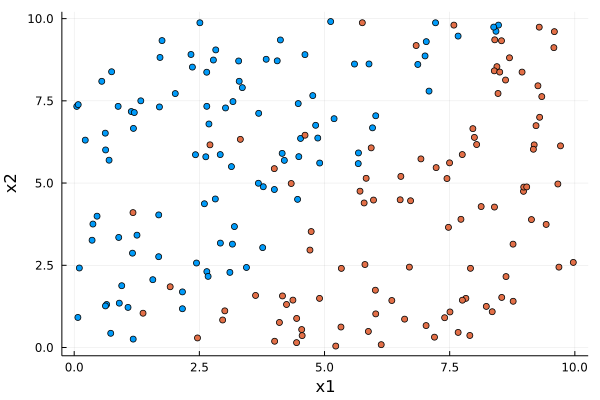
\includegraphics[width=0.95\columnwidth]{graphics/Chap13SeparatingHyperplanes/SoftMarginData.png}%
\caption[]{Raw data where there is some overlap between the two classes. This is quite typical in practice.}    
\label{fig:soft_margin_01}
\end{figure}

In such cases, the best one can do is to seek a hyperplane that roughly minimizes the number of data points that are misclassified. This is done with a ``soft margin classifier'', where the hard constraint in \eqref{eq:MaxMarginCommonConstraint} is replaced with 
\begin{equation}
\label{eq:SoftMarginCommonConstraint}
       \ell_i(w^\top \bar{x}_i)-\xi_i \geq 1, ~~1 \le i \le n,
\end{equation}
where for $\xi_i >1$, a data point is allowed to be in the wrong class. To make sure this is the exception rather than the rule, we try to make the vector $\xi$ have small norm. This gives rise to the QP
\begin{equation}\begin{aligned}
  \underset{\xi,w}{\rm min  } ~~~ \frac{1}{2} \xi^\top \xi & + \frac{\lambda}{2} a^\top a \\
\left[\begin{array}{c}  \ell_1 ~\bar{x}_1^\top \\ \vdots \\  \ell_n ~\bar{x}_n^\top \end{array} \right] \left[\begin{array}{c} a \\ a_0 \end{array} \right] &\geq \left[\begin{array}{c} 1 -\xi_1 \\ \vdots \\  1 -\xi_n \end{array} \right],
\end{aligned}\end{equation}
where $\lambda >0$ trades off the separation property versus the soft margin.  



\begin{figure}[hb!]%
\centering
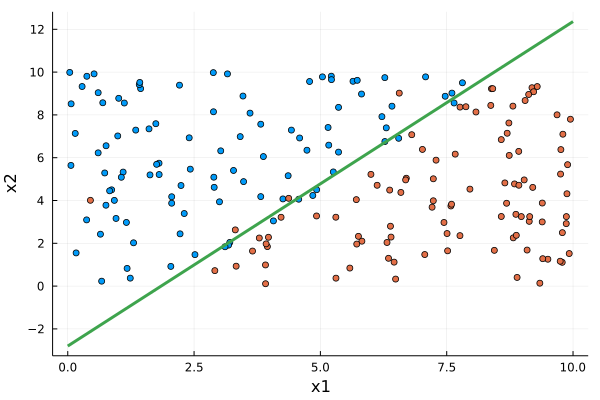
\includegraphics[width=0.95\columnwidth]{graphics/Chap13SeparatingHyperplanes/SoftMarginSeperated.png}%
\caption[]{A ``separating'' hyperplane that allows a few missclassifications.}    
\label{fig:soft_margin_02}
\end{figure}


\begin{lstlisting}[language=Julia,style=mystyle]
# generate a dataset
N = 100 # Desired number of data points in each class
n = 2*N # Total number of points
k1 = 0; # number of 1
k2 = 0; # number of -1
X = zeros(n,2); # input matrix
ell = zeros(n,1); # target values
i = 1;
while minimum([k1 k2]) < N
    x = rand(1,2) * 10.;
    # separating line is x2 = 1.5 x1 + 0.4
    y = (x[2] - 1.5 * x[1] - 0.4)
    # generate target values
    if (y > -3.5) && k1 < N
        ell[i] = 1;
        X[i,:] = x;
        k1 += 1;
        i += 1;
    elseif (y < 3.5) && k2 < N
        ell[i] = -1;
        X[i,:] = x;
        k2 += 1;
        i += 1;
    end
end

# Class +1 IDs
class1_id = ell.== 1;

using Plots
gr() # Set the backend to GR

plot(X[class1_id[:],1], X[class1_id[:],2], seriestype = :scatter, legend = false)
plot!(X[.!class1_id[:],1], X[.!class1_id[:],2], seriestype = :scatter)
xlabel!("x1")
ylabel!("x2")
\end{lstlisting}
\textbf{Output} 
See Fig.~\ref{fig:soft_margin_01}.

\begin{lstlisting}[language=Julia,style=mystyle]
# Define problem data using the native Julia form for the QP solver
m = 3;
lambda = 1; # tunable parameter (called hyperparameter because it's not like w the parameter of our model)
P = sparse([lambda*(zeros(m,m) + I) zeros(m,n); zeros(n,m) (zeros(n,n) + I)]);
q = zeros(n+m,1);
A = [-sparse([ell ell ell] .* [X ones(n,1)]) -(zeros(n,n) + I); zeros(n,m) (zeros(n,n) + I)]
l = [zeros(n,1) .- Inf; zeros(n,1)];
u = [-ones(n,1); zeros(n,1) .+ Inf];

# Crate OSQP object
prob = OSQP.Model()

# Setup workspace and change alpha parameter
OSQP.setup!(prob; P=P, q=q[:], A=A, l=l[:], u=u[:])

# Solve problem
results = OSQP.solve!(prob);

w_line = -results.x ./ results.x[2];

x_line = collect(0:0.1:10)
y_line = w_line[1] * x_line .+ w_line[3]
plot!(x_line, y_line, lw=3)

\end{lstlisting}
\textbf{Output} 
See Fig.~\ref{fig:soft_margin_02}.


\begin{lstlisting}[language=Julia,style=mystyle]
zeta = results.x[4:end]
@show maximum(zeta)
@show minimum(zeta)
println(" ")
println("These are misclassified data points or they are outliers in your data set.")
indicesBigZeta=findall(x->x>1,zeta) # These are misclassified 
\end{lstlisting}
\textbf{Output} 
\begin{verbatim}
maximum(zeta) = 3.2141869873099136
minimum(zeta) = 2.3479433444366696e-8
 
These are misclassified data points or they are outliers in your data set.
13-element Vector{Int64}:
  18
  43
  56
  66
  87
  94
 131
 144
 150
 194
 195
 196
 198
\end{verbatim}
\begin{figure}[hb!]%
\centering
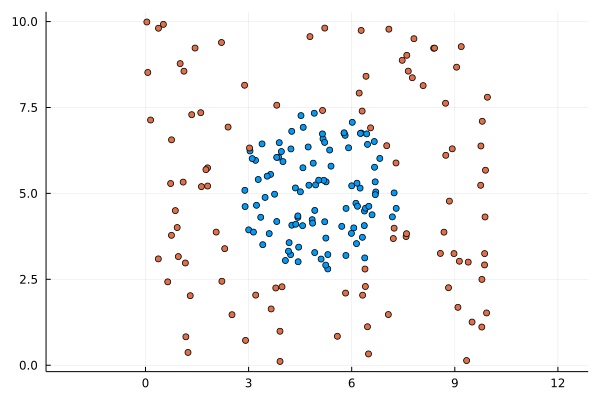
\includegraphics[width=0.95\columnwidth]{graphics/Chap13SeparatingHyperplanes/GaussiamSoftMargin01.png}%
\caption[]{Raw data where it seems impossible to separate the data with a hyperplane.}    
\label{fig:Gaussian_soft_margin_01}
\end{figure}

We next look at a problem where it seems impossible to separate the data with a hyperplane, such as shown in Fig.~\ref{fig:Gaussian_soft_margin_01}. The trick is to add more features to the data by adding nonlinear terms. For example, instead of working in $\real^2$ with $[x_1~~~x_2]$ as features, we could work in $\real^5$ with the feature vector being
$$\left[\begin{array}{c} x_1\\ x_2\\ 1 \\ (x_1)^2 \\ x_1 x_2 \\ (x_2)^2 \end{array} \right]. $$
This gives more possibilities for the data to be separated. The above choice is motivated by the blue data seemingly belonging to a disc. We are not obliged, however, to use monomials. In Project 2, we learned about radial basis functions, or RBFs for short. As shown in Fig.~\ref{fig:Gaussian_soft_margin_02}, this provides a lot of flexibility for separating the data into two classes.

\begin{figure}[hb!]%
\centering
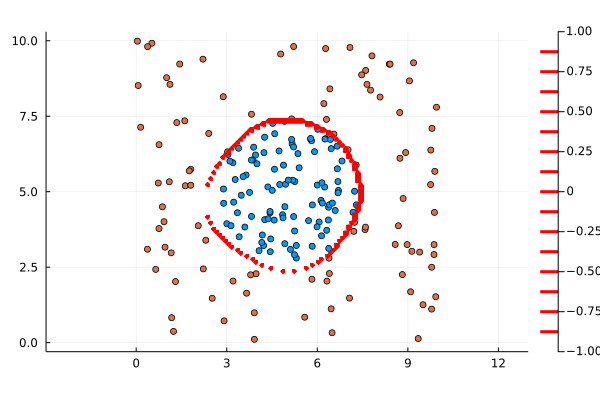
\includegraphics[width=0.95\columnwidth]{graphics/Chap13SeparatingHyperplanes/GaussiamSoftMargin02.png}%
\caption[]{A Gaussian soft-margin classifier, where radial basis functions have been used to lift the data to  $\real^{n+2}$, where $n$ is the number of data points. When we evaluate the sign of the classifier on our data in $\real^2$, we obtain an approximation of a circle. In $\real^{202}$, there is a separating hyperplane. }    
\label{fig:Gaussian_soft_margin_02}
\end{figure}



\begin{lstlisting}[language=Julia,style=mystyle]
# generate a dataset
N = 100 # Desired number of data points in each class
n = 2*N # Total number of points
k1 = 0; # number of 1
k2 = 0; # number of -1
X = zeros(n,2); # input matrix
ell = zeros(n,1); # target values
i = 1;
while minimum([k1 k2]) < N
    x = rand(1,2) * 10.;
    y = (x[1]-5)^2 + (x[2]-5)^2;
    # generate target values
    if (y < 5.5) && k1 < N
        ell[i] = 1;
        X[i,:] = x;
        k1 += 1;
        i += 1;
    elseif (y > 4) && k2 < N
        ell[i] = -1;
        X[i,:] = x;
        k2 += 1;
        i += 1;
    end
end

# Class +1 IDs
class1_id = ell .== 1;

using Plots
gr() # Set the backend to GR

plot(X[class1_id[:],1], X[class1_id[:],2], seriestype = :scatter, legend=false)
plot!(X[.!class1_id[:],1], X[.!class1_id[:],2], seriestype = :scatter)
plot!(aspectratio=:equal)
\end{lstlisting}
\textbf{Output} 
See Fig.~\ref{fig:Gaussian_soft_margin_01}.


\begin{lstlisting}[language=Julia,style=mystyle]
# Functions from Project 2

# Radial basis function
s = 1;
rbf(x, z, s) = exp.(-norm(x-z)^2 / (2*s^2));

function calc_phi_row(x, z, s) 
    NumBasisElements = size(z,1) + 2
    # plus two above because we also include a x1 and x2
    phi_row = zeros(1,NumBasisElements)
    phi_row[1:2] = [x[1]  x[2]]    
    for i in 3:NumBasisElements
        phi_row[i] = rbf(x, z[i-2,:], s)
    end     
    return phi_row
end

function regressor_matrix(X, centers, s)
    ### BEGIN SOLUTION
    N = size(X,1)
    M = size(centers,1)
    Phi = Array{Float64, 2}(undef, N, M+2)
    for i = 1:N
        Phi[i, :] = calc_phi_row(X[i,:], centers, s)
    end
    return Phi
    ### END SOLUTION 
end
\end{lstlisting}


\begin{lstlisting}[language=Julia,style=mystyle]
# Define problem data
m = n+2;
lambda = 0.01; # tunable parameter (called hyperparameter because it's not like w the parameter of our model)
P = sparse([lambda*(zeros(m,m) + I) zeros(m,n); zeros(n,m) (zeros(n,n) + I)]);
q = zeros(n+m,1);
Phi = regressor_matrix(X,X,s);
A = sparse([-\ell.*Phi -(zeros(n,n) + I); zeros(n,m) (zeros(n,n) + I)])
l = [zeros(n,1) .- Inf; zeros(n,1)];
u = [-ones(n,1); zeros(n,1) .+ Inf];

# Create OSQP object
prob = OSQP.Model()

# Setup workspace and change alpha parameter
OSQP.setup!(prob; P=P, q=q[:], A=A, l=l[:], u=u[:])

# Solve problem
results = OSQP.solve!(prob);
\end{lstlisting}


\begin{lstlisting}[language=Julia,style=mystyle]
# create test data
x1 = 0:0.1:10;
x2 = 0:0.1:10;
X1 = zeros(length(x2),length(x1));
X2 = zeros(length(x2),length(x1));
for j=1:length(x1)
    for i=1:length(x2)
        X1[i,j]= x1[j]
        X2[i,j]= x2[i]
    end
end
X_test = [X1[:] X2[:]];
# get model weights
alpha = results.x[1:m,:]
# query
Phi_test = regressor_matrix(X_test,X,s);
Y_test = Phi_test * alpha;

plot(X[class1_id[:],1], X[class1_id[:],2], seriestype = :scatter)
plot!(X[.!class1_id[:],1], X[.!class1_id[:],2], seriestype = :scatter)

Z = sign.(reshape(Y_test, (length(x2), length(x1)))); # +1 or -1
# plot the margins
contour!(x1, x2, Z, lw=3, color=:red, legend=false) # The contour line separates class -1 from class +1 
plot!(aspectratio=:equal)
\end{lstlisting}
\textbf{Output} 
See Fig.~\ref{fig:Gaussian_soft_margin_02}.\\

\begin{remark} What is the classifier for the data? It is 
$$ \begin{aligned} \alpha & = results.x[1:m,:] \\
{\rm Classifier}(x) &= (calc\_phi\_row(x, X, s)*\alpha)[1]  \end{aligned}$$   
The data from $\real^2$ have been lifted to $\real^{n+2} = \real^{202}$ via
$${\rm Classifier}(x) = {\rm Classifier}(x_1, x_2) = \left[ \begin{array}{ccccc}x_1 & x_2 & e^{-\frac{||x-z_1||^2}{2} }& \cdots & e^{-\frac{||x-z_n||^2}{2}} \end{array} \right] \left[ \begin{array}{c} \alpha^\ast_a \\ \alpha^\ast_b \\ \alpha^\ast_1 \\ \vdots \\ \alpha^\ast_n  \end{array} \right], $$
where $z_1, z_2, \ldots, z_n$ are the two-dimensional data points in Fig.~\ref{fig:Gaussian_soft_margin_01}. The code block below shows that there are no misclassified points! 
\end{remark}


\begin{lstlisting}[language=Julia,style=mystyle]
alpha = results.x[1:m,:]
Classifier(x) = (calc_phi_row(x, X, s)*alpha)[1]

for i in 1:n
    test = Classifier(X[i,:])
    if sign(test) != ell[i]
        @show [i ell[i] test] # misclassified data points
    end    
end
\end{lstlisting}
\textbf{Output} 
Nothing! There are no misclassified data points!


\section{Orthogonal Projection}
\label{sec:OrthogonalProjection}

We extend the importance of the dot product (aka, inner product) by showing its fundamental role in least squares problems. \\

\subsection{Orthogonal Projection for Subspaces}
 \vspace*{0.2cm}
\begin{figure}[hbt!]
\centering
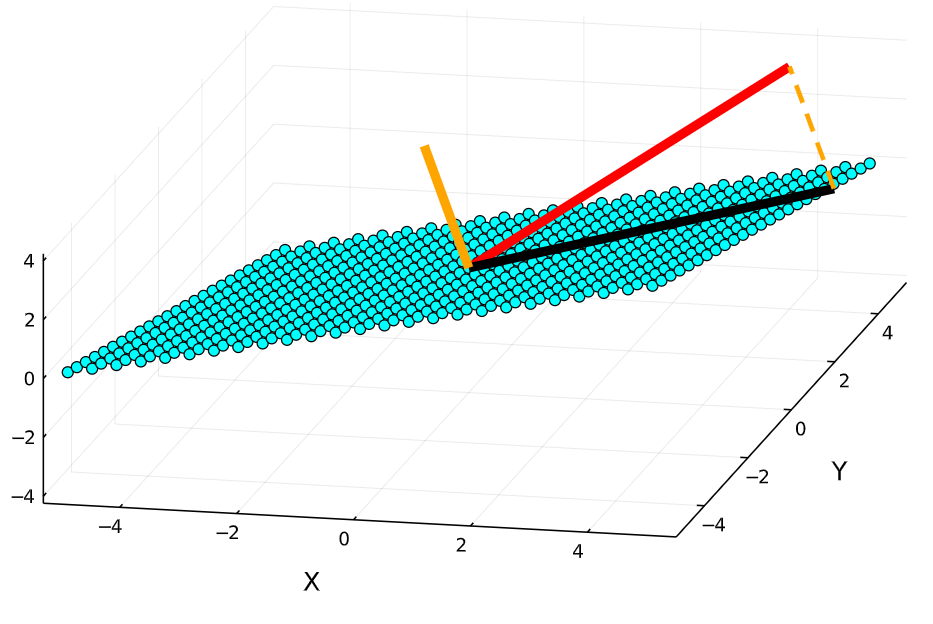
\includegraphics[width=0.8\textwidth]{graphics/Chap13SeparatingHyperplanes/orthogonalProjectionImage.png}
\caption[]{A vector (in red) is orthogonally projected (in black) onto a subspace (in cyan). The error vector (in solid orange) is orthogonal to the plane. This characterizes the orthogonal projection process. The vector in dashed orange is the error vector drawn to highlight that the error forms a right angle with the projection of the vector. } 
\label{fig:SimpleOrthongalProjection}
\end{figure}

\vspace*{0.2cm}

\begin{tcolorbox}[title=\Large \textbf{Review}]
Consider the vector space $\real^n$, which we view as the set of all $n \times 1$ column vectors of real numbers. Let $v, w \in \real^n$ and let $V\subset \real^n$ be a subspace.
\begin{itemize}
    \item  $v \bullet w := v^\top w$.
    \item  $w\bullet v = v \bullet w$.
    \item $v \perp w \iff v \bullet w = 0$.
    \item $v \perp w \implies ||v + w||^2 = ||v||^2 + ||w||^2$ (Pythagorean Theorem).
    \item Let $\{u_1, u_2, \ldots, u_m\}$ be a basis for $V$. Then Gram-Schmidt produces an \textbf{orthogonal basis} that also satisfies, for all $1\le k \le m$,
    $$ \spanof{u_1, u_2, \ldots, u_k} = \spanof{v_1, v_2, \ldots, v_k}.$$
    Moreover, by the simple step of adding normalization to Gram-Schmidt, we can assume that $\{v_1, v_2, \ldots, v_m\}$ is an \textbf{orthonormal basis} for $V$.
\end{itemize}
\end{tcolorbox}

%%\subsection{Best Approximation by a Subspace}

% \textbf{Definition} Let $S \subset \real^n$ be a subset. Its \textbf{orthogonal complement} is defined as 
% \begin{equation}
%     \label{eq:orthongalComplement}
%     S^\perp:=\{ x\in \real^n~|~ x\perp y,~~\text{for all}~~y \in S \}.
% \end{equation}

% \begin{example}
% \label{ex:OrthogComple01}
% We first consider sets that consist of single vectors. 
% $$ S_1=\left\{  \begin{bmatrix} 1 \\ 2 \end{bmatrix} \right\} \subset \real^2~~\text{and}~~ S_2=\left\{  \begin{bmatrix} 1 \\ 1\\ 1\end{bmatrix} \right\} \subset \real^3.$$
% \end{example}

% \textbf{Solution:}

% \begin{align*}
%     S_1^\perp&:= \{ x\in \real^2~|~ x\perp \begin{bmatrix} 1 \\ 2 \end{bmatrix} \} \\
%     &= \{ x\in \real^2~|~ \begin{bmatrix} x_1 \\ x_2 \end{bmatrix} \bullet \begin{bmatrix} 1 \\ 2 \end{bmatrix} =0 \} \\
%      &= \{ x\in \real^2~|~ x_1 + 2 x_2 =0 \} \\
%      & = \spanof{\left[ \begin{array}{r} 2 \\ -1 \end{array} \right] }.
% \end{align*}

% \begin{align*}
%     S_2^\perp&:= \{ x\in \real^3~|~ x\perp \begin{bmatrix} 1 \\ 1 \\1 \end{bmatrix} \} \\
%     &= \{ x\in \real^3~|~ \begin{bmatrix} x_1 \\ x_2 \\ x_3\end{bmatrix} \bullet \begin{bmatrix} 1 \\ 1 \\ 1 \end{bmatrix} =0 \} \\
%      &= \{ x\in \real^2~|~ x_1 +  x_2 + x_3=0 \} \\
%      & = \spanof{ \left[ \begin{array}{r} 1 \\ -1 \\ 0 \end{array} \right],  \left[ \begin{array}{r} 0 \\ 1 \\ -1 \end{array} \right] }.
% \end{align*}
% \Qed


% \begin{example}
% \label{ex:OrthogComple01}
% We next consider a set that consist of two vectors. 
% $$ S_3=\left\{  \begin{bmatrix} 1 \\ 1\\ 1\end{bmatrix},  \left[ \begin{array}{r} 2 \\ -1 \\ 1 \end{array} \right] \right\} \subset \real^3.$$
% \end{example}

% \textbf{Solution} Add more examples as needed. 

% \Qed

\begin{tcolorbox}[sharp corners, colback=green!30, colframe=green!80!blue, title=\textbf{\large Projection Theorem: The Super Tool that Solves all Least Squares Problems}]

Let $V$ be a subspace of $\real^n$ and let $x_0$ be an arbitrary point in $\real^n$. Then there exists a unique vector $x^\ast \in V$ such that 
$$ ||x_0-x^\ast||=\min\limits_{x \in V} ||x_0-x||;$$
as before, we denote this vector by $x^\ast = \argmin\limits_{x \in V} || x_0 - x||$ or by $x^\ast = \argmin\limits_{x \in V} || x_0 - x||^2$. Moreover, the solution to the least squared error problem is uniquely characterised by
\begin{equation}
    \label{eq:ProjThmCharacterization}
    x^\ast = \argmin\limits_{x \in V} || x_0 - x||^2 \iff \left(x_0-x^\ast\right) \perp V ~~\text{and}~~x^\ast \in V.
\end{equation}
 The vector $x_0 - x^\ast$ is called the \textbf{error vector}. The vector $x^\ast$ is called the \textbf{orthogonal projection of $\mathbf{x_0}$ onto $\mathbf{V}$} precisely because the error vector is orthogonal to $V$. Recalling the Pythagorean Theorem, we have that 
 $$||x_0 - x^\ast||^2 + || x^\ast||^2 = ||x_0||^2; $$
 once again emphasizing that $x^\ast$, $x_0 - x^\ast$, and $x_0$ form a ``generalized right triangle''.
\end{tcolorbox}

\vspace*{0.2cm}

You already know one way to compute $x^\ast$ from the Projection Theorem! Really? Yes, Gram Schmidt. If $x_0 \in V$, the solution to the problem is trivial, namely $x^\ast = x_0$, because then the error is zero, which is as small as it gets. Hence, suppose $x_0\not \in V$ and let $\{u_1, u_2, \ldots, u_m \}$ be a basis for $V$. Then we leave it to you to show that
$$ x_0 \not \in V \iff x_0 \not \in \spanof{u_1, u_2, \ldots, u_m } \iff \{u_1, u_2, \ldots, u_m, x_0\}~~\text{is linearly independent}.$$
We apply Gram-Schmidt\footnote{We do not assume normalization, but you can also do that.} to the set $\{u_1, u_2, \ldots, u_m, x_0\}$. The last step gives that
$$v_{m+1} = x_0 -\sum_{k=1}^m \frac{x_0 \bullet v_k}{v_k \bullet v_k}v_k,$$
and moreover, we know that 
$$v_{m+1} \perp \spanof{v_1, v_2, \ldots, v_m} =V.$$
Hence, by the Projection Theorem, 
\begin{equation}
\label{eq:ComputeOrthognalProjectionGS}
 \boxed{x^\ast =  \sum_{k=1}^m \frac{x_0 \bullet v_k}{v_k \bullet v_k}v_k,} 
\end{equation}
because $ x_0 - x^\ast = v_{m+1}$ and $v_{m+1} \perp V$.\\

\textbf{Remark:} Once we know that \eqref{eq:ComputeOrthognalProjectionGS} is true, we can simply apply Gram-Schmidt to any basis of $V$ to produce an orthogonal basis and then apply  \eqref{eq:ComputeOrthognalProjectionGS}. If we produce an \textbf{orthonormal basis}, then we know that $v_k \bullet v_k=1$ and the formula simplifies to 
\begin{equation}
\label{eq:ComputeOrthognalProjectionGS02}
\boxed{x^\ast = \sum_{k=1}^m \left(x_0 \bullet v_k \right) v_k =  \sum_{k=1}^m \left< x_0 ,  v_k \right> v_k,}  
\end{equation}
where we have recalled our alternative notation for an inner product.\\

A second way to compute the solution follows from \eqref{eq:ProjThmCharacterization} and leads to the \textbf{Normal Equations}. Once again, let $\{u_1, u_2, \ldots, u_m \}$ be any basis for $V$. Because we know that $x^\ast \in V$, we can pose 
\begin{equation}
    \label{eq:xstarInV}
    x^\ast = \alpha_1 u_1 + \alpha_2 u_2 + \cdots + \alpha_m u_m 
\end{equation}
as a linear combination of basis vectors for $V$ and seek the conditions on the coefficients $\alpha_1, \alpha_2, \ldots, \alpha_m$ so that
$$x_0 - x^\ast \perp V. $$
You can quickly convince yourself that 
$$x_0 - x^\ast \perp V \iff x_0 - x^\ast \perp u_k, 1 \le k \le m. $$
The above constitutes $m$-equations, one for each $k$, and leads to the famous Normal Equations,
\begin{equation}
    \label{eq:NormalEquations}
    \underbrace{\left[\begin{array}{cccc}
u_1 \bullet u_1 & u_1\bullet u_2 & \cdots & u_1 \bullet u_m \\
u_2 \bullet u_1 & u_2\bullet u_2 & \cdots & u_2 \bullet u_m \\
\vdots & \vdots & \ddots & \vdots \\
u_m \bullet u_1 & u_m\bullet u_2 & \cdots & u_m \bullet u_m \
    \end{array}  \right]}_{G} \underbrace{\begin{bmatrix}
    \alpha_1\\\alpha_2\\ \vdots \\ \alpha_m
    \end{bmatrix}}_{\alpha} = \underbrace{\begin{bmatrix}
    u_1 \bullet x_0\\ u_2 \bullet x_0 \\ \vdots \\ u_m \bullet x_0
    \end{bmatrix}}_{\beta}.
\end{equation}
The matrix $G$ is called the \textbf{Gram matrix} and is invertible if, and only if, the set $\{ u_1, u_2, \ldots, u_m\}$ is linearly independent. We note the the $ij$-entry of it is 
$$G_{ij}=u_i \bullet u_j = u_i^\top u_j. $$
We'll let you work out that if you take a basis for $V$ that is orthogonal, then $G$ is a diagonal matrix, and if you take an orthonormal basis for $V$, then $G$ is the identity matrix! \\

We summarize the various solutions in the following:
\vspace*{0.2cm}

\begin{tcolorbox}[title=\textbf{Computing the Solution Given by the Projection Theorem}]
Let $V$ a subspace of $\real^n$ and $x_0 \in \real^n$ be given. Then  $x^\ast = \argmin\limits_{x \in V} || x_0 - x||^2$, the orthogonal projection of $x_0$ onto $V$, can be computed by
\begin{itemize}
\item $x^\ast = \sum_{k=1}^m \left(x_0 \bullet v_k \right) v_k $ if $\{ v_1, \cdots, v_m\}$ is an \textbf{orthonormal basis} for $V$; 
    \item $x^\ast = \sum_{k=1}^m \frac{x_0 \bullet v_k}{v_k \bullet v_k}v_k $  if $\{ v_1, \cdots, v_m\}$ is an \textbf{orthogonal basis} for $V$; 
    \item  $x^\ast = \alpha_1 u_1 + \alpha_2 u_2 + \cdots \alpha_m u_m $, where $G \alpha = \beta$ are the Normal Equations given in \eqref{eq:NormalEquations}, if $\{ u_1, \cdots, u_m\}$ is \textbf{any basis} for $V$.
\end{itemize}
\end{tcolorbox}

You instructors use all of these forms of the solution at various times when solving problems. 
%a=[-.4;.4;1]; V=nullspace(a*a'); w=4*[1;1;1]
\vspace*{0.2cm}

\begin{example}
\label{ex:OrthongoanlProjectionSimpleExample} 
We'll warm up on a simple example. Consider a subspace given by $V= \spanof{u_1, u_2}$, where
$$u_1=\left[ \begin{array}{r} 1.0 \\ 1.0 \\ 0.0 \end{array} \right], u_2=\left[ \begin{array}{r} 2.5 \\ 0.0 \\ 1.0 \end{array} \right]. $$
Compute the orthogonal projection of $x_0 = \left[ \begin{array}{r} 4.0 \\ 4.0 \\ 4.0 \end{array} \right]$ onto $V$. Moreover, compute
$$x^\ast = \argmin\limits_{x \in V} || x_0 - x||^2  $$
in at least two different ways. 
\end{example}

\textbf{Solution A:} We apply the normal equations
\begin{align*}
G &= \left[ \begin{array}{rr} u_1^\top u_1 & u_1^\top u_2 \\ u_2^\top u_1 & u_2^\top u_2 \end{array} \right] = \left[ \begin{array}{rr} 2.00 & 2.50 \\
2.50 & 7.25  \end{array} \right] \\
\\
\beta&=  \left[ \begin{array}{r} u_1^\top x_0 \\
u_2^\top x_0 \\\end{array} \right]= \left[ \begin{array}{r} 8.00 \\
14.00 \\\end{array} \right] \\
\\
G \alpha & =  \beta \implies \alpha= \left[
\begin{array}{c}
2.79 \\
0.97 \\
\end{array}
\right]\\
\\
x^\ast & = \alpha_1 u_1 + \alpha_2 u_2 = \left[
\begin{array}{c}
5.21 \\
2.79 \\
0.97 \\
\end{array}
\right].
\end{align*}
The results are illustrated in Fig.~\ref{fig:SimpleOrthongalProjection}.

\vspace*{0.2cm}
\textbf{Solution B:} We find an orthonormal basis for $V$ and apply \eqref{eq:ComputeOrthognalProjectionGS02}. We use Gram-Schmidt with normalization and find that
$V=\spanof{v_1, v_2}$, for 
$$v_1=
\left[
\begin{array}{r}
0.707 \\
0.707 \\
0.000 \\
\end{array}
\right]
~~\text{and}~~v_2=
\left[
\begin{array}{r}
0.615 \\
-0.615 \\
0.492 \\
\end{array}
\right].
 $$
 Hence, 
 $$x^\ast = \left(v_1^\top x_0 \right) v_1 + \left( v_2^\top x_0 \right) v_2  = 5.657 v_1 + 1.969 v_2 = \left[
\begin{array}{c}
5.212 \\
2.788 \\
0.970 \\
\end{array}
\right].  $$

\vspace*{0.2cm}
\textbf{Solution C:} Finally, we use an orthogonal basis for $V$ and apply \eqref{eq:ComputeOrthognalProjectionGS}. For our orthogonal basis, we apply Gram-Schmidt without normalization and obtain
$V=\spanof{v_1, v_2}$, for 
$$v_1=\left[
\begin{array}{c}
1.0 \\
1.0 \\
0.0\\
\end{array}
\right]
~~\text{and}~~v_2=
\left[
\begin{array}{r}
1.25 \\
-1.25 \\
1.00 \\
\end{array}
\right].
 $$
 Hence, 
 $$x^\ast = \frac{v_1^\top x_0 }{v_1^\top v_1} v_1 + \frac{v_2^\top x_0}{v_2^\top v_2} v_2  = 4.0 v_1 + 0.970 v_2 = \left[
\begin{array}{c}
5.212 \\
2.788 \\
0.970 \\
\end{array}
\right].  $$
\Qed.

\vspace*{0.2cm}

In this next example, we apply the Normal Equations to our very first least squares problem in \eqref{eq:ThmLeastSqaredErrorSolution}! The example is essentially a proof showing how to derive our original result from the Projection Theorem. \textcolor{red}{Trigger Warning: This is not for the faint of heart. Your instructors did not learn this as undergraduates, much less, first-year undergraduates!} If you skip the example, we highly recommend the summary that follows it.

\begin{example}
\label{ex:OrthongoanlProjectionforAxEquals}
Consider a system of linear equations $Ax=b$, where $A$ is $n \times m$ and its columns are linearly independent. Define 
$$ V:=\colspanof{A}.$$
Relate the following two least squares problems
\begin{itemize}
    \item $x^\ast = \argmin\limits_{x \in \real^m} || Ax-b||^2$
    \item $v^\ast =\argmin\limits_{v \in V}||b-v||^2,$
\end{itemize}
where we renamed the solution of the second optimization problem as $v^\ast$ to avoid confusion later on.  (Yikes! It must not be easy.) 
\end{example}

\textbf{Solution}
The first least squares problem is well known to us from \eqref{eq:ThmLeastSqaredErrorSolution}, which we repeat here for clarity
$$x^\ast = \argmin\limits_{x \in \real^m} || Ax-b||^2 \iff A^\top A x^\ast =A^\top b,$$
which we've always interpreted as the least squared error solution to over determined equations. Moreover, this provided the basis for our work on regression, which was, we recall, pretty awesome. \\

The second least squares problem is still kind of a mystery to us. If we believe what we were were told about its solution, then $v^\ast$ is the orthogonal projection of $b$ onto the column span of the matrix $A$. What could that possibly mean? Well, let's find out!\\

We write $A$ out in terms of its columns, $A = \left[ \begin{array}{cccc}A_1 & A_2 & \ldots & A_m \end{array}\right]$, so that
$$\colspanof{A} = \spanof{A_1, A_2, \ldots, A_m}.$$
When we compute the Gram matrix, we recall that $G_{ij} =  A_i \bullet A_j = A_i^\top A_j$, which is precisely the $ij$-entry of $A^\top A$, and thus
$$G =  A^\top A, $$
an amazing coincidence! We'll let you work out a few examples to see that this is true or we'll let you work out a proof! Moreover, when we compute the $i$-th entry of $\beta$ we obtain
$\beta_i = A_i \bullet b = A_i^\top b$, so that
$$\beta = A^\top b, $$
another amazing coincidence! (Or, perhaps not!). Finally, we note (aka, ``let you work out'') that
$$\sum_{k=1}^m \alpha_k A_k = A \alpha, $$
which should either be setting off alarms in your head because this many coincidences should never happen.....except for a reason! \textbf{The two least squares problems are really one and the same problem.}\\

To see this, we summarize what we have
\begin{itemize}
    \item $v^\ast =  \argmin\limits_{v \in \colspanof{A}}||b-v||^2 \iff  \left(A^\top A \alpha = A^\top b~~\text{and}~~v^\ast = A \alpha \right).$
    \item $x^\ast = \argmin\limits_{x \in \real^m} || Ax-b||^2 \iff A^\top A x^\ast =A^\top b.$
    \item Hence, $\alpha = x^\ast$, and $v^\ast = A x^\ast$ is the orthogonal projection of $b$ onto the column span of $A$. 
    \item By projecting $b$ onto the column span of $A$, we have that 
    $$v^\ast \in \spanof {A_1, A_2, \ldots, A_m},$$
    and hence $A x = v^\ast$ has a solution. Kind of clever, isn't it! 
    \item The fact that all of that is being accomplished by the simple equation $A^\top A x^\ast =A^\top b$ is one of the \textbf{Wonders of Linear Algebra}. It's a really beautiful subject and we hope you will want to learn more about it. There is so much more to it than what we have covered in the main parts of this book.
\end{itemize}
\Qed

\textbf{Remark:} This is a heavy result, so it will take you some time to wrap your head around it. The main message is that the Projection Theorem and the Normal Equations are your main tools when you approach new least squares problems. They have extensions to settings that you cannot even imagine right now. But they are always there, providing theoretical and computational support for solving least squares problems of so many kinds.

\vspace*{.2cm}

\textbf{It is clear why we did not broach this result in our main treatment of least squares problems. We would have sent you running and screaming for any course but ROB 101!}

\vspace*{0.2cm}

\begin{tcolorbox}[title=\textbf{Summary of the Previous Example}]
Suppose that $\{u_1, u_2, \ldots, u_m \}$ is a basis for a subspace $V \subset \real^n$ and $x_0 \in \real^n$. Form a matrix $U$ with the  basis vectors as its columns, that is,
$$U= \left[ \begin{array}{cccc}u_1 & u_2 & \ldots & u_m \end{array}\right]. $$
Then the solution to 
 $x^\ast = \argmin\limits_{x \in V} || x_0 - x||^2 $ is given by
 $$\boxed{U^\top U \alpha^\ast = U^\top x_0,~ x^\ast = U \alpha^\ast.} $$
\end{tcolorbox}

\subsection{Orthogonal Projection onto Linear Varieties (translations of subspaces)}
Let $V\subset \real^n$ be a subspace (of any dimension) and $v_c \in \real^n$ be a point. We define the linear variety, $W:=v_c + V$, as the translation of the subspace $V$ by the vector $v_c$. Though it is not very common, one can consider the \textbf{orthogonal projection} of a vector $x_0\in \real^n$ onto the linear variety $W$. The key idea is to once again pose a best approximation problem and to consider the properties that define its solution, by properly interpreting the Projection Theorem. 

\begin{tcolorbox}[title=\textbf{Small Extension of the Projection Theorem}]
 Consider a linear variety $W:=v_c + V$, where  $V\subset \real^n$ is a subspace (of any dimension) and $v_c \in \real^n$ is a point. For $x_0 \in \real^n$ arbitrary, the following are equivalent:
 \begin{enumerate}
 \renewcommand{\labelenumi}{(\alph{enumi})}
\setlength{\itemsep}{.2cm}
     \item $w^\ast = \argmin\limits_{w \in W} ||x_0 -w||^2.$
     \item $w^\ast =v^\ast +v_c$, where $ v^\ast= \argmin\limits_{v \in V} ||(x_0-v_c) - v||^2.$
       \item $w^\ast =v^\ast +v_c$, where $v^\ast \in V$ and $\big( (x_0 - v_c) - v^\ast \big) \perp V$ 
     \item  $w^\ast \in W$ and $\big( (x_0 - v_c) - (w^\ast-v_c) \big) \perp V$. 
     \item  $w^\ast \in W$ and $(x_0-w^\ast) \perp V$.
 \end{enumerate}
 The last condition, (e), emphasizes that the error term, $x_0-w^\ast$, is orthogonal to $V$. 
 The second condition, (b), shows how to compute $w^\ast$: orthogonally project $x_0-v_c$ onto $V$, and then add $v_c$ to the answer.\\
 
 We gave (a) through (e) in the order we would use them in a proof, were we to give it! The order we chose should help you to see how each fact is a small variation of the previous one, while going straight from (a) to (e) would be rather daunting.
\end{tcolorbox}



\begin{example}
\label{ex:exampleFrom445} Compute the orthogonal projection of $x_0 = \left[ \begin{array}{r} 4.0 \\ 4.0 \\ 4.0 \end{array} \right]$ onto $W := v_c + V$, where $V= \spanof{u_1, u_2}$, 
$$u_1=\left[ \begin{array}{r} 1.0 \\ 1.0 \\ 0.0 \end{array} \right], u_2=\left[ \begin{array}{r} 2.5 \\ 0.0 \\ 1.0 \end{array} \right] $$ 
and $v_c = \left[ \begin{array}{r} 1.0 \\ 2.0 \\ 3.0 \end{array} \right]$. Moreover, compute the norm of the error term, $x_0 - w^\ast$, which we now know is the distance of $x_0$ from the linear variety $W$.
\end{example}

\textbf{Solution:} Our strategy is we form $\overline{x}_0:=x_0 - v_c = \left[ \begin{array}{r} 3.0 \\ 2.0 \\ 1.0 \end{array} \right]$ and compute $v^\ast$, its orthogonal projection onto $V$. We then have $w^\ast = v^\ast + v_c$ is the orthogonal projection of $x_0$ onto $W=V+v_c$.\\

Using our work from Example~\ref{ex:OrthongoanlProjectionSimpleExample}, Solution B, we have that
$V=\spanof{v_1, v_2}$, for 
$$v_1=
\left[
\begin{array}{r}
0.707 \\
0.707 \\
0.000 \\
\end{array}
\right]
~~\text{and}~~v_2=
\left[
\begin{array}{r}
0.615 \\
-0.615 \\
0.492 \\
\end{array}
\right].
 $$
 Hence, 
 $$v^\ast = \left(v_1^\top \overline{x}_0 \right) v_1 + \left( v_2^\top \overline{x}_0 \right) v_2  = -1.5 v_1 -0.182 v_2 = \left[
\begin{array}{r}
-1.727 \\
-1.273 \\
-0.182 \\
\end{array}
\right].  $$
Hence, 
$$w^\ast = v^\ast + v_c = \left[
\begin{array}{r}
-0.727 \\
0.727 \\
2.818 \\
\end{array}
\right].
 $$

We next compute 
$$d(x_0,W):=\min\limits_{w \in W} ||x_0 - w || = ||x_0 - w^\ast|| = 2.08893$$

\Qed
\vspace*{0.2cm}

\begin{example}
\label{ex:exampleFrom445B} As a natural continuation of Example~\ref{ex:exampleFrom445}, we note that $W\subset \real^3$ is a hyperplane. Compute the signed distance of $x_0$ from $W$. 
\end{example}

\textbf{Solution:} We need to write the hyperplane as the zero set of a function $y:\real^3 \to \real$, where
$$y(x)=a \bullet(x-v_c), $$
and $a\in \real^3$ has norm one. Once again, appealing to Gram-Schmidt, we have that
$$ a=
\left[
\begin{array}{r}
-0.348 \\
0.348 \\
0.870 \\
\end{array}
\right].
$$
Doing the required computation yields that the signed distance is 
$$y(x_0)  = -2.08893.$$
Comparing to our result in Example~\ref{ex:exampleFrom445}, we see that
$$y(x_0)=-d(x_0, W), $$
in other words, the terminology ``signed distance'' is justified!
\Qed 


  